In this chapter I present the surface stress and adhesion energy data collected for two types of silicone with various stiffnesses. We first used Gelest to obtain our preliminary data and tune the operation of our device. We then switched to Dow-Corning to continue more extensive measurements. 


\section{Organosilicon Polymer Chemistry}
\label{section:polychem}
\emph{MUST MOVE THIS. I should definitely talk about what the heck Silicone actually is, and what we're really using, and frankly why gels are stretchy. I think that I should say something in the introduction, and maybe designate an appendix if I want to go more in depth.} 

PDMS, or Poly-Dimethyl-Siloxane, is a commonly used gel in the field of soft condensed matter. The gel is composed of a polymer network of crosslinkers, as well as a second polymer in the fluid phase. When stretched, the configuration of the system changes such that the tangled crosslinkers begin to unwind and untangle. From a statistical mechanics perspective, this decreases the configurational entropy, thus increasing the free energy. \emph{Which free energy though? I think this is what we're covering next in 302...Also I got this from that unpublished review article}

Below (Fig. \ref{fig:DMS-V31}) is the chemical structure for the vinyl-terminated PDMS (Gelest) that comprises the fluid phase. 
% Set chemical bonds length
\setatomsep{20pt}

% -------------From chemfig manual, useful macro--------------------
\newcommand\setpolymerdelim[2]{\def\delimleft{#1}\def\delimright{#2}}
\def\makebraces(#1,#2)#3#4#5{%
	\edef\delimhalfdim{\the\dimexpr(#1+#2)/2}%
	\edef\delimvshift{\the\dimexpr(#1-#2)/2}%
	\chemmove{
		\node[at=(#4),yshift=(\delimvshift)]
		{$
			\left\delimleft
			\vrule height\delimhalfdim depth\delimhalfdim width0pt
			\right.
			$};
		\node[at=(#5),yshift=(\delimvshift)]
		{$
			\left.
			\vrule height\delimhalfdim depth\delimhalfdim width0pt
			\right\delimright_{\rlap{#3}}
			$};
	}%
}

%PDMS DMS-V31 Figure
\begin{figure}[h!]
	\centering
	\scalebox{1.75}{
		\setpolymerdelim()
		
		\chemfig{H_2C=C(-[-3]H)--[@{op,0}]Si(-[2]CH_3)(-[6]CH_3)-O--[@{cl,0}]Si(-[2]CH_3)(-[6]CH_3)-C(-[7]H)=CH_2}
		
		\makebraces(20pt,20pt){$\!\!n$}{op}{cl}
	}
	\label{fig:DMS-V31}
	\caption[DMS-V31]{Divinyl-terminated Polydimethylsiloxane (DMS-V31)}
\end{figure}

The crosslinker for the system is a trimethylsiloxane terminated 25-35\% methylhydrosiloxane - dimethylsiloxane copolymer. The crosslinker is much shorter on average than the PDMS, containing roughly 20-30 repeating monomer groups. The single hydrogen on the methylhudrosiloxane is weakly bound, and can be replaced by one of the hydrogen atoms in the PDMS. This bonding happens over and over again, creating the long twisted chains that create the mesh network of the gel. Increasing density of crosslinkers provides an easy and controllable method to vary the gel's stiffness.

%PDMS Crosslinker HMS-301 Figure
\begin{figure}
	\centering
	\scalebox{1.75}{
		\setpolymerdelim()
		%the [@{op,offset}] and [@{cl,offset}] are for the giant parentheses macro function.
		\chemfig{H_3C-Si(-[2]CH_3)(-[6]CH_3)-O--[@{op,0}]Si(-[2]H)(-[6]CH_3)-O-[@{cl,.5}]-[@{op2,.5}]Si(-[2]CH_3)(-[6]CH3)-O--[@{cl2,0}]Si(-[2]CH_3)(-[6]CH_3)-CH_3}
		
		\makebraces(20pt,20pt){$\!\!m$}{op}{cl}
		\makebraces(20pt,20pt){$\!\!n$}{op2}{cl2}
	}		
	\label{fig:HMS-301}
	\caption[HMS-301]{Trimethylsiloxane terminated 25-35\% methylhydrosiloxane ($m$) - dimethylsiloxane ($n$). This is the crosslinker. \emph{I could make that lone H red to help make clearer where the crosslinker bonding is happening. Thoughts?}}
\end{figure}

\begin{table}[h!]
	\caption[PDMS ratios Characterization]{PDMS gel characterization}
	\begin{center}
		\begin{tabular}{|c||c||c|}
			\hline
			Mix Ratio (A\&B) & Young's Modulus (kPa) & Sol Fraction (\%)\\
			\hline
			$7.5:1$ & $2.5 \,\pm\, 0.1$ & 65.2\\
			\hline
			$9:1$ & $5.0 \, \pm\, 0.1$  & 64.7\\
			\hline
			$11:1$ & $10.0 \,\pm\, 1$  & 63.7\\
			\hline
		\end{tabular}
	\end{center}
	\label{tab:recipes}
\end{table}


\section{Preliminary Data}
Because Figure \ref{fig:2017natcomfig} was obtained using Dow-Corning silicone gel, our intention from the start was to use this material in our adhesion based measurements. Because the material was back-ordered, we used Gelest instead while we calibrated the process. I present this preliminary data because it shows clear incremental steps of evidence that the surface stress for the substrate is increasing under strain.  

\subsection{Standard Candles}
Not only do we measure the depth and radii for a range of spheres, but we also measure a select few spheres at every strain. This allows us to track how any given sphere is changing, increasing our confidence that the shift in $\Upsilon$ and W is not just an artifact of noise. Below is the side profile for Gelest 9:1 ($\text{E}=6.3$ kPa). Notice how the profile shifts noticeably upwards to be flattened when the substrate is stretched. This shift is expected if the surface stress is increasing (see equation \ref{THEeqn}).

\begin{figure}
	\centering
	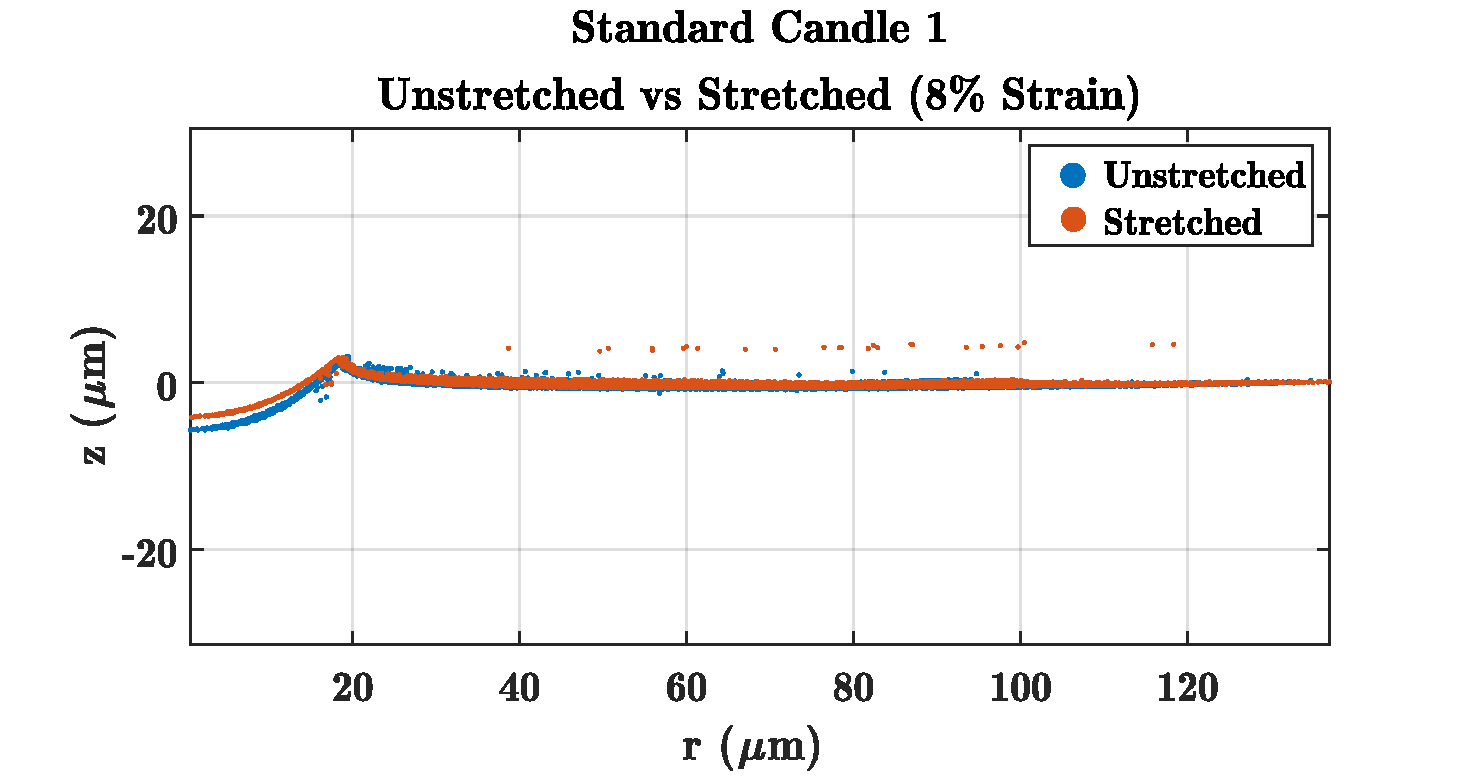
\includegraphics[width=\linewidth]{Chapters/Figures/sc1_unstretched_v_8ml}
	\caption[Side Collapse Comparison]{The side profile of the same sphere before and after stretch. Notice how after stretching, the sphere's indentation into the substrate is shallower. Substrate is Gelest 9:1 ($\text{E}=6.3$ kPa).}	
	\label{fig:sc1unstretchedv8ml}
\end{figure}
\todo[inline,color=yellow]{Change the font of the figure to CMU extra}
\begin{figure}
	\centering
	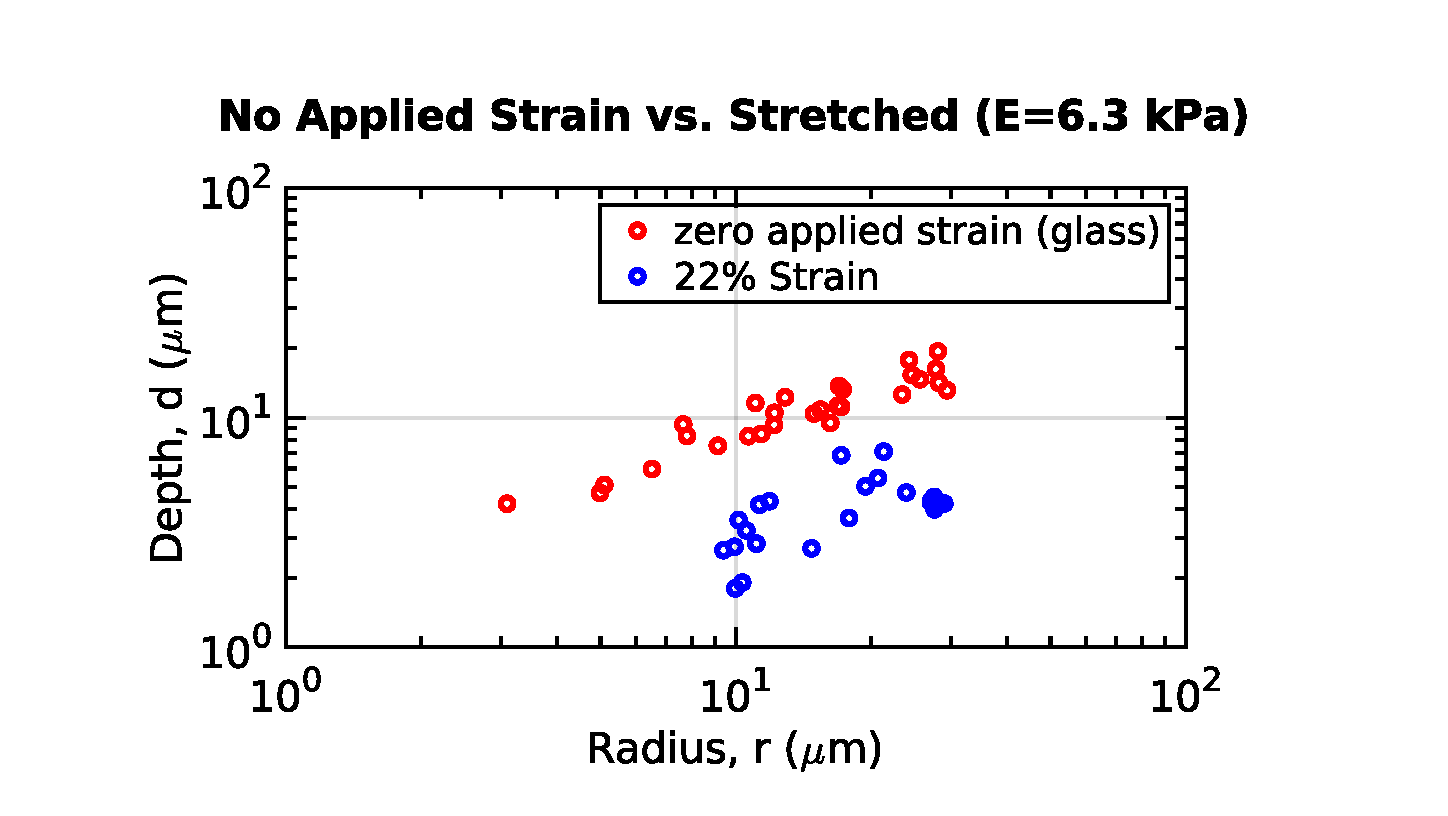
\includegraphics[width=\linewidth]{Chapters/Figures/glass_vs_stretched_190218}
	\caption[Glass vs. Stretched d vs. R]{For Gelest 9:1. The silicone under strain (blue) on average sink less deep into the silicone than the same silicone spun on glass (zero applied strain)}

	\label{fig:glassvsstretched190218}
\end{figure}

\section{Data}
\emph{go get that sweet DC d vs r goodness}